%\clearpage
% \FloatBarrier
\appendix
In this supplement, we (1) show additional experiment results on small Video LLM and multiple-view video understanding (Section~\ref{experiment}); (2) describe additional implementation details (Section~\ref{implementation}); (3) include additional visualization of the question-answering results (Section~\ref{visualization}).
% and (4) provide further discussion of setting of using multiple patches and potential future work (Section~\ref{discussion}). 
%We hope that this document will complement our main paper. 

% For sections, figures, tables, and equations, we use numbers (e.g., Sec. 1) to refer to the main paper and capital letters (e.g., Sec. A) to refer to this supplement.
\begin{table*}[t]  
\centering  
\scalebox{0.77}{
\begin{tabular}{lc|c|cccc|c|c}  
\toprule
       \multirow{2}{*}{Method}      & AVSD~\cite{alamri2019audiovisualsceneawaredialog}  &AVQA~\cite{yang2022avqa}&\multicolumn{4}{c|}{MUSIC-AVQA~\cite{Li2022Learning}}  & \multirow{2}{*}{TFLOPs} & \multirow{2}{*}{Total / Trainable Params} \\
                                    & CIDEr                                              & Acc. &Audio Acc. & Visual Acc. & Audio-Visual Acc.  & Overall Acc. & & \\
    \midrule
    \multicolumn{3}{l}{\it \small\textbf{Zero-shot LMMs} } \\
     %CAT-7B ~\cite{ye2024catenhancingmultimodallarge}             & 79.0 & -  & -  & -    & -    & 48.6 & -      & - \\
     LLaVA-OV-0.5B~\cite{li2024llava}                             & 65.1 & 77.4 & \textcolor{gray}{60.0} & 57.1 & 48.5 & 52.8 & 8.01 & 0.9B~/~-\\
     LLaVA-OV-7B~\cite{li2024llava}                               & 70.6 & 85.6 & \textcolor{gray}{68.8} & 70.6 & 52.8 & 60.4 & 98.53 & 8.2B~/~-\\
     \midrule
     \multicolumn{3}{l}{\it \small\textbf{Task-specific models} } \\     
     %MTN~\cite{Le_2019}                                           & 98.5  & -  & - & - & -  &  - &-  & -\\
     %COST~\cite{pham2022videodialogconversationobjects}           & 108.5 & -  & - & - & -  &  - &-  & - \\
     %VALOR~\cite{chen2023valorvisionaudiolanguageomniperceptionpretraining} & -  & - & - & -  & -&  78.9 & - & - \\
     %VAST~\cite{chen2023vast} & -  & - & - & -  & -&  80.7 & - & - \\
     %PSTP-Net~\cite{li2023progressive} & -  & 90.2 & - & -  & -&  - & - & - \\
     %CAT-7B-FT ~\cite{ye2024catenhancingmultimodallarge}          & - & 92.0 & \textcolor{gray}{\textbf{84.9}} & 86.1 & \textbf{83.2} &    \textbf{84.3} & -  & - \\ %0.6492%
     LLaVA-OV-0.5B-FT                                             & 117.6  & 86.4 & \textcolor{gray}{69.6} & 76.3 & 62.8 &  67.6  & 8.01 & 0.9B~/~35.2M \\
     LLaVA-OV-7B-FT                                               & 124.9  & 90.8 & \textcolor{gray}{75.4} & 89.3 & 72.3 &  77.4  & 98.53 & 8.2B~/~161.5M \\
     \midrule
     
     PAVE-0.5B (w/ audio)                                          & 134.5 &  90.4  & \textcolor{gray}{77.3} & 89.8  & 74.1 & 78.8 & 8.08 & 0.9B~/~41.4M   \\
     PAVE-7B   (w/ audio)                                          & 152.9 & 93.8 & \textcolor{gray}{79.7} & 93.0 & 78.0 &  82.3 & 98.63 & 8.2B~/~170.5M \\ \bottomrule

\end{tabular}
}


% \vspace{-1mm}
\caption{Additional result of PAVE on the audio-visual understanding tasks with audio as additional information. 
\vspace{-1mm}
}  
\label{tab:video_audio_understanding_appendix}  
\end{table*}  

\begin{table*}[t]  
\centering  
\scalebox{0.8}{
\begin{tabular}{lccccc|c|c|c}  
\toprule
\multirow{2}{*}{Method}                                          & \multicolumn{5}{c|}{ScanQA~\cite{azuma_2022_CVPR}} & SQA3D\cite{ma2022sqa3d} & \multirow{2}{*}{TFLOPs} & \multirow{2}{*}{Total / Trainable Params}\\
                                                                 & C     & B-4 & M     & R    & EM@1 & EM@1     &&            \\ 
    \midrule
    \multicolumn{6}{l}{\it \small\textbf{Zero-shot LMMs}} \\
     %VideoChat2-7B~\cite{li2024mvbenchcomprehensivemultimodalvideo} & 49.2  & 9.6 & 9.5   & 28.2 & 19.2 & 37.3 & - & - \\
     LLaVA-OV-0.5B~\cite{li2024llava}                            & 17.2  & 1.2 & 13.7  & 18.4 & 0.2 \textcolor{gray}{(28.0)} & 0.8 \textcolor{gray}{(43.0)} & 8.01 & 0.9B~/- \\
     LLaVA-OV-7B~\cite{li2024llava}                              & 91.0  & 5.3 &  18.2 & 45.9 & 26.7 \textcolor{gray}{(44.3)} & 8.3 \textcolor{gray}{(50.7)} &98.53 & 8.2B / - \\
    \midrule
    \multicolumn{6}{l}{\it \small\textbf{Task-specific models}} \\
     %Scene-LLM-7B~\cite{fu2024scenellmextendinglanguagemodel}       &  80.0 & 12.0 & 16.6 & 40.0 & 27.2 & 54.2 & - & - \\
     %LLaVA-3D-7B~\cite{zhu2024llava3dsimpleeffectivepathway}        &  91.7  & 14.5 & \textbf{20.7} & \textbf{50.1} & 27.0 \textcolor{gray}{(45.0)} & 55.6 \textcolor{gray}{(57.6)} & - & - \\%14.35%
      % LLaVA-3D (re-eval)                                         &  83.8  & 10.8 & 16.7 & 42.6 & 25.7 \textcolor{gray}{(45.1)}            &  & - & - \\
      LLaVA-OV-0.5B-FT  & 70.5 & 6.5 & 14.3 & 36.9 & 20.5 \textcolor{gray}{(36.3)}  & 44.1 \textcolor{gray}{(45.7)} & 8.01 & 0.9B~/~35.2M\\
      LLaVA-OV-7B-FT    & 95.1 & 13.5 & 19.1 & 47.4 & 27.4 \textcolor{gray}{(46.3)} & 55.8 \textcolor{gray}{(58.1)} & 98.53 & 8.2B / 161.5M \\
    \midrule
     PAVE-0.5B (w/ 3D info)                                       & 84.2 & 13.1 & 17.0 & 42.1 & 23.1 \textcolor{gray}{(40.0)}&  51.1 \textcolor{gray}{(52.8)} & 8.13 & 0.9B~/~41.4M\\
     PAVE-7B   (w/ 3D info)                                       & 103.4 & 16.0 & 19.9 & 49.0 & 29.1 \textcolor{gray}{(48.5)} & 59.0 \textcolor{gray}{(61.4)} & 98.68 & 8.2B / 170.5M\\ \bottomrule
     

\end{tabular}
}
% \vspace{-1mm}
\caption{Additional result of PAVE on the 3DQA tasks with 3D information as additional information.
}  
\vspace{-1mm}
\label{tab:3d_qa_understanding_appendix}  
\end{table*}  



\begin{table*}[t]  
\centering  
\scalebox{0.72}{
\begin{tabular}{l|ccccc|c|c}  
\toprule
% \multirow{2}{*}{Method}   & \multicolumn{4}{c|}{VideoMME~\cite{fu2024video}} & \multicolumn{4}{c|}{MVBench~\cite{li2023mvbench}} & \multirow{2}{*}{MLVU~\cite{zhou2025mlvubenchmarkingmultitasklong}}  & \multirow{2}{*}{FLOPs(TB)} & \multirow{2}{*}{Total / Trainable Params}  \\
     Method                               & ActivtityNet-QA & EgoSchema & NextQA & PerceptionTest & VideoMME (w-subs) & FLOPs (TB) & Total / Trainable Params \\ 
    \midrule
     LLaVA-OV-0.5B~\cite{li2024llava}     & 50.5            & 26.8      & 57.2   & 49.2            & 43.5 & 8.01 & 0.9B~/~- \\
     LLaVA-OV-7B~\cite{li2024llava}       & 56.6            & 60.1      & 79.4   & 57.1            & 61.5 & 98.53 & 8.2B~/~- \\
     \midrule
     PAVE-0.5B (w/ video feature)         & 50.6 & 27.1  &    56.1 & 48.8 & 48.6 & 8.08  & 0.9B~/~41.4M  \\
     PAVE-7B   (w/ video feature)         & 57.1 & 57.4  &    79.6 & 56.0 & 62.9 & 98.63 & 8.2B~/~170.5M \\ \bottomrule

\end{tabular}
}
% \vspace{-1mm}
\caption{Result of PAVE on the additional benchmarks in enhanced video understanding setting. PAVE uses densely sampled video frames as additional information. 
\vspace{-1mm}
}  
\label{tab:general_video_understanding_appendix}  
\end{table*}  




\section{Additional Experiment Results} \label{experiment}
% \subsection{The Experiments with Small Language Model.}
\subsection{Results with small Video LLM} 

We now present additional experiment results of PAVE with LLaVA-OneVision 0.5B models for audio-visual QA and 3D QA. 
Table~\ref{tab:video_audio_understanding_appendix} and Table~\ref{tab:3d_qa_understanding_appendix} show the results. PAVE consistently improves the 0.5B and 7B Video LLM's performance by a large margin across both settings. 
% Specifically, we observed a significant performance gap between LLaVA-OV-FT and PAVE. 
This indicates that PAVE effectively leverages additional information when adapting pre-trained Video LLMs into new settings. 

\subsection{Results on Enhanced Video Understanding} 

We present PAVE's result on additional benchmarks in the enhanced video understanding setting. 
% These results were omitted from the main paper due to space limit.
Table~\ref{tab:general_video_understanding_appendix} shows PAVE's results in the enhanced video understanding setting with additional benchmarks. PAVE demonstrates a substantial performance gain on VideoMME (w-subtitles). However, we observe only marginal or no improvement on ActivityNet-QA, EgoSchema, NextQA, and PerceptionTest. We hypothesize that this discrepancy may be due to: (1) domain shift—our training data primarily consists of third-person view videos, which may lead to a performance drop in EgoSchema, and (2) the nature of the benchmark questions, which may not require densely temporal information for reasoning.





\begin{table}[t]  
\centering
% \vspace{-1em}
\resizebox{0.98\linewidth}{!}{
\begin{tabular}{lccc}  
\toprule
       Model                    & Acc. & FLOPs (TB) &  Total / Trainable Params \\
     \midrule
     \multicolumn{4}{l}{\it \small\textbf{Zero-shot LMMs}} \\
     LLaVA-OV-0.5B    &  23.6   & 8.01  & 0.9B~/ -   \\
     LLaVA-OV-7B   &  23.6    & 98.53  & -    \\
     \midrule
     \multicolumn{4}{l}{\it \small\textbf{Task-specific models}} \\
     LLaVA-OV-0.5B-FT             & 28.2     & 8.01  & 0.9B~/~35.2M  \\
     LLaVA-OV-7B-FT             & 29.8     & 98.53  & 8.2B / 161.5M  \\
     TimeSFormer (Ego+Exo)* ~\cite{grauman2024ego}      & 43.7    & -  &   -  \\
     % TimeSFormer (Ego)        & 47.2  & -  &   -  \\
     % TimeSFormer (Ego+Exo)* ~\cite{grauman2024ego}      & 43.7    & -  &   -  \\
     % CAT-7B-FT                  & -   & 92.0 & -  &   -  \\
     \midrule
     PAVE-0.5B                & 32.4           & 8.15 & 0.9B~/~41.4M \\ 
     PAVE-7B                  & 44.2  & 98.70 & 8.2B / 170.5M \\ 
     % PAVE-AVQA                & -   & \textbf{93.8} & 8.00 & 8.2B / 170.4M\\ 
     \bottomrule

\end{tabular}
}
\vspace{-2mm}
%\caption{Result of multi-view video recognition on Ego-Exo4D
\caption{Performance of PAVE on multi-view video understanding with Ego-Exo4D Demonstrator Proficiency benchmark. LLaVA-OV-7B-FT refers to directly fine-tuning the LLaVA-OneVision on the training set. Our model achieves state-of-the-art performance by only adding a small amount of parameters and FLOPs. * means this baseline may use more training data than PAVE because some of the videos are unavailable to us.} 
\label{tab:ego_exo_videos_appendix}  
\end{table}


\subsection{Results on Multi-view Video Understanding} \label{section_res_multi_view_video}
\noindent\textbf{Motivation and task set up.}
Understanding human activity from video is crucial in many real-world applications, such as augmented reality and robotic learning. Based on the perspective, videos can be broadly classified into ego-centric and exo-centric views. Ego-centric videos capture first-person interactions, focusing on close-up hand-object interactions, while exo-centric videos provide a third-person perspective, recording full-body postures and the surrounding environment. Both perspectives are essential for comprehensive human action understanding. 
Different from the audio-visual QA and 3D QA, where the side-channel information comes from other modalities, in this context, PAVE regards exo-centric videos as side-channel information and integrates it with ego-centric video to adapt the Video LLMs for multi-view video understanding.

\medskip
\noindent\textbf{Training data.} 
We use the training set from the Ego-Exo4D demonstrator proficiency estimation benchmark~\cite{grauman2024ego} as our training data, which consists of 1,904 question-answer pairs. Each pair is associated with one ego-centric video and four exo-centric videos. The task requires the model to classify human action proficiency into one of four categories: Novice, Early Expert, Intermediate Expert, or Late Expert, based on both ego- and exo-centric videos. However, only 1,656 question-answer pairs include the corresponding videos, as the videos for the remaining pairs could not be downloaded due to privacy issues.


\medskip
\noindent\textbf{Implementation details.}
Considering the exo- and ego-centric videos are synchronized along the temporal axis, we sample 32 frames for each of the exo-centric videos. To keep the encoding procedure consistent between the ego- and exo-video, we use the same preprocessing of the LLaVA-OneVision to reshape and crop the video frames. We use SigLIP~\cite{zhai2023sigmoidlosslanguageimage} as the visual encoder and it encodes and downsamples each frame into 196 tokens. We pre-extract the exo-video feature tokens offline to accelerate the training. 
We build PAVE on top of LLaVA-OneVision~\cite{li2024llava} and train the model for 2 epochs.


\medskip
\noindent\textbf{Evaluation benchmark.} 
We use the validation set of the Ego-Exo4D~\cite{grauman2024ego} demonstrator proficiency estimation benchmark for evaluation and report accuracy as the metric. It contains 466 questions and each of the questions is paired with 1 ego-centric video and 4 exo-centric videos.
% what metriec we use 
% how many question we have 
% what is the qiestion look like 

\medskip
\noindent\textbf{Baselines.}
% baseline from the egoexo
% baseline by fineting the model
We use the TimeSFormer (Ego+Exo) from Ego-Exo4D~\cite{grauman2024ego} as our baseline. We also include a baseline that directly fine-tunes the LLaVA-OneVision with LoRA on the training set without using the exo-centric videos, denoted as LLaVA-OV-7B-FT. This baseline allows us to assess whether PAVE can effectively utilize supplementary information.

\medskip
\noindent\textbf{Results.} Table~\ref{tab:ego_exo_videos_appendix} shows the results of PAVE. Compared with the LLaVA-OV-7B-FT, PAVE-7B achieves about 14.4\% improvement by adding only 9M parameters and 0.17 TFLOPs during inference. This big improvement indicates that the exo-centric videos provide crucial additional information for human action understanding.
Moreover, PAVE achieves state-of-the-art performance on the demonstrator proficiency estimation benchmark, substantiating that  PAVE can adapt a pre-trained Video LLM to an unseen setting by leveraging supplementary information. 

% \begin{table}[h!]  
% \centering
% % \vspace{-1em}
% \resizebox{0.98\linewidth}{!}{
% \begin{tabular}{lccc}  
% \toprule
%        Model                    & Acc. & FLOPs (TB) &  Total / Trainable Params \\
%      \midrule
%      LLaVA-OV-7B (Zero-shot)    &  23.6    & 98.53  & -    \\
%      LLaVA-OV-7B-FT             & 29.8     & 98.53  & 8.2B / 161.5M  \\
%      % TimeSFormer (Ego)        & 47.2  & -  &   -  \\
%      TimeSFormer (Ego+Exo)* ~\cite{grauman2024ego}      & 43.7    & -  &   -  \\
%      % CAT-7B-FT                  & -   & 92.0 & -  &   -  \\
%      \midrule
%      PAVE-7B (w/ Exo-videos)             & \textbf{44.2}  & 98.70 & 8.2B / 170.5M \\ 
%      % PAVE-AVQA                & -   & \textbf{93.8} & 8.00 & 8.2B / 170.4M\\ 
%      \bottomrule

% \end{tabular}
% }
% \vspace{-2mm}
% %\caption{Result of multi-view video recognition on Ego-Exo4D
% \caption{Performance of PAVE on multi-view video understanding with Ego-Exo4D Demonstrator Proficiency benchmark. LLaVA-OV-7B-FT refers to directly fine-tuning the LLaVA-OneVision on the training set. Our model achieves state-of-the-art performance by only adding a small amount of parameters and FLOPs. * means this baseline may use more training data than PAVE because some of the videos are unavailable to us.} 
% \label{tab:ego_exo_videos}  
% \end{table}


\section{Implementation and Experiment Details} \label{implementation}
We first describe the general implementation detail of the PAVE in Section~\ref{pave_inple}. Then, we describe the experiment details for 3 settings considered in the main paper, including audio-visual QA (Section~\ref{avqa}), 3DQA (Section~\ref{3dqa}), and enhancing video QA (Section~\ref{enhanced_video_qa}). We also demonstrate how we calculate the Flops for the model in Section~\ref{flops_calc}.

\subsection{Implementation Detail of PAVE} \label{pave_inple}


Inside the temporal-aligned cross-attention layer, we add rotary position embedding to the query and key tokens. Specifically, we apply different rotary positional embedding according to the layout of side-channel tokens $\mathbf{z}^s$. We mainly consider two types of $\mathbf{z}^s$: (a) $\{\mathbf{z}^s\}$ includes both spatial and temporal dimensions, such as tokens from video backbones or from a 3D backbone; and (b) $\{\mathbf{z}^s\}$ only contains temporal dimension, such as audio tokens. For the first case, we will add 3D rotary positional embedding (along the temporal, height, and width dimensions). For the second case, we will only add rotary positional embedding along the temporal axis. After cross-attention, we use a two-layer MLP, followed by a layer norm. 
After the PAVE layers, we add another two-layer MLP, followed by a layer norm, as the adapter. We initialize the $\gamma$ in the layer norm to zero. 
% For all experiments, we use a learning rate of 2e-5 and a batch size of 32 to adapt the pre-trained Video LLM.




%%%%%%%%%%%%%%%%%%%%%%%%%%%%%%%%% AVQA
% all other things including some of the implementation details.




\subsection{Audio-Visual QA}\label{avqa}
In this setting, the input of the PAVE has two parts: (1) the visual tokens $\mathbf{z}^v$ from the Video LLM's visual encoder, and (2) the audio tokens $\mathbf{z}^s$ from a side-channel signal encoder.

\medskip
\noindent \textbf{Visual Encoder.} For $\mathbf{z}^v$, we follow the default setting used in LLaVA-OneVision~\cite{li2024llava}. We uniformly sample 32 frames from the video and use the same preprocessing of the LLaVA-OneVision to reshape and crop the video frames. We use SigLIP~\cite{zhai2023sigmoidlosslanguageimage} as the visual encoder and it encodes and downsamples each frame into 196 tokens. 


\medskip
\noindent \textbf{Side-Channel Signal Encoder.}
For $\mathbf{z}^s$, we follow the pre-processing step of ImageBind~\cite{girdhar2023imagebind}, which resamples the audio at 16KHz. 
% In order to fit into the design of the Audio Spectrogram Transformer~\cite{gong2021astaudiospectrogramtransformer}, we split the audio tokens along the temporal axis into multiple groups with each group containing 1024 tokens. We later concatenate the encoded features of all groups along the temporal axis. Audio Spectrogram Transformer will down-sample the temporal dimension by 16 and generate about 6 tokens per second with token dimension 768. 
We segment the audio into overlapping 2-second clips with a 1-second stride and encode each clip using the audio encoder of ImageBind. This process generates a 1024-dimensional audio token for every 1 second of the audio signal.
Since we do not fine-tune the audio encoder, we extract the audio feature tokens offline in order to accelerate the training.

\medskip
\noindent \textbf{Network Architecture.} For the PAVE design, we use 2 cross-attention layers with hidden dimension 512 and have 4 attention heads. 
% After the cross-attention, we add 2 layers of MLP and a layer normalization layer, in which $\gamma$ is initialized as 0 at the beginning of the training. 
For LoRA layers in the LLM, we use LoRA$\_r$ = 64 and LoRA$\_\alpha$ = 16. 

\medskip
\noindent \textbf{Training Details.}
For training, we use AdamW~\cite{loshchilov2019decoupledweightdecayregularization} optimizer with a linear warmup using the first 3\% of iterations. We use the cosine annealing learning rate during the training. We set the base learning rate as 2e-5 and the batch size as 32. All the experiments are run on 2 A100 80G GPUs. 

\medskip
\noindent\textbf{Training data.} We choose the open-end QA dataset AVSD~\cite{alamri2019audiovisualsceneawaredialog}, and closed-end QA dataset AVQA~\cite{yang2022avqa} and Music-AVQA~\cite{Li2022Learning} as training dataset. AVSD contains 79k question-answer pairs across 7,985 videos with each paired 10 questions. AVQA has 40k question-answer pairs coupled with 40k Videos. Music-AVQA consists of 32k question-answer pairs and 9277 videos.

\medskip
\noindent\textbf{Evaluation benchmark.} We follow the protocol in previous works~\cite{ye2024catenhancingmultimodallarge, pham2022videodialogconversationobjects} to evaluate PAVE. For AVSD, we use the AVSD@DSTC7 test split and report CIDEr score as the metric. This benchmark consists of 1,000 audio-visual questions.
We use COCO API~\cite{lin2015microsoftcococommonobjects} to calculate the CIDEr score between the model predictions and the ground truth answers. 
For AVQA, we evaluate PAVE on the eval split and report the accuracy as the metric. This benchmark contains 17k questions that require reasoning based on audio and visual information.
For Music-AVQA, we evaluate PAVE on the test split and report the accuracy as the metric. This benchmark contains 9185 questions, which can be categorized into visual, audio, and audio-visual questions.
% Additionally, we calculate the model inference FLOPs at the prefilling stage using LLM-Viewer~\cite{yuan2024llm}.






%%%%%%%%%%%%%%%%%%%%%%%%%%%%%%%%%%%% 3d QA

\subsection{3DQA} \label{3dqa}
In this setting, the input of the PAVE consists of two parts: (1) the visual tokens $\mathbf{z}^v$ from the Video LLM's visual encoder, and (2) the 3D tokens $\mathbf{z}^s$ from a side-channel signal encoder.

\medskip
\noindent \textbf{Visual Encoder.} For $\mathbf{z}^v$, we use the same setting as the one in Section~\ref{avqa}. 

\medskip
\noindent \textbf{Side-Channel Signal Encoder.} For encoding the side-channels information into $\mathbf{z}^s$, we utilize the 3D encoder which contains two parts 1. a visual encoder which encodes the RGB frames into visual feature tokens. 2. a spatial embedding that adds the encoded 3D information on the visual feature tokens. We uniformly extract 32 RGB-D frames from the scan and use ViT~\cite{dosovitskiy2021imageworth16x16words} to extract the visual features from the RGB frames. We then add spatial embeddings to visual features following the LLaVA-3D~\cite{zhu2024llava3dsimpleeffectivepathway} by making use of the depth information and the camera pose. It generates 576 tokens for each frame, with a token dimension of 1024. We pre-extract the 3D feature to accelerate the training.


\medskip
\noindent \textbf{Network Architecture and Training Details.} For the PAVE design and the training configuration, we use the same hyper-parameters used in Section~\ref{avqa}.

% \noindent\textbf{3DQA Implementation details.}
% To encode 3D information, we follow the LLaVA-3D~\cite{zhu2024llava3dsimpleeffectivepathway} that adds spatial embeddings to the visual tokens generated by ViT~\cite{dosovitskiy2021imageworth16x16words}. Since the videos are relatively short in the 3D setting, we evenly sample 32 RGB-D frames from the scanning videos. We send the RGB-D frame with the camera pose into the ViT backbone and generate 18432 tokens per scan. 
% We build PAVE on top of LLaVA-OneVision\cite{li2024llava}. We train the PAVE with ScanQA / SQA3D training set when evaluating PAVE performance on ScanQA / SQA3D, respectively. For ScanQA experiments, we train PAVE for one epoch on its training set, whereas for SQA3D, we train PAVE for two epochs.

\medskip
\noindent\textbf{Training data.} For 3D QA tasks, we consider ScanQA~\cite{azuma_2022_CVPR} and SQA3D~\cite{ma2022sqa3d}. ScanQA and SQA3D contain 25K and 26K training question-answer pairs, respectively. They share the same scanning data set which contains 562 3D scanning from ScanNet~\cite{dai2017scannet}. 


\medskip
\noindent\textbf{Evaluation benchmark.} We report our model performance on the ScanQA validation set, which contains 4,675 questions covering both object position reasoning and object recognition, and the SQA3D test set with 3519 questions, which consists of 5 different types of questions.
Following previous work~\cite{zhu2024llava3dsimpleeffectivepathway}, we report the CIDEr (C), BLEU-4 (B-4), METEOR (M), ROUGE(R), and top-1 Exact Match (EM@1) metrics on ScanQA and report EM@1 on SQA3D. We use the evaluation pipeline set up by LLaVA-3D to evaluate our model on ScanQA and SQA3D. 
% We also calculate the model inference FLOPs at the prefilling stage using LLM-Viewer~\cite{yuan2024llm}.




%%%%%%%%%%%%%%%%%%%%%%%%%%% multi view %%%%%%%%%%%%%%%%%%

% \subsection{Multi-view Video Understanding} \label{multi_view}
% In this setting, the input of the PAVE consists of two parts: (1) the ego-centric visual tokens $\mathbf{z}^v$ from the Video LLM's visual encoder which encodes the ego-centric video, and (2) the exo-centric the visual tokens $\mathbf{z}^s$ from the Side-Channel signal encoder which encodes the exo-centric videos.


% \medskip
% \noindent \textbf{Visual Encoder.} For $\mathbf{z}^v$, we use the same setting as the one in Section~\ref{avqa}. 

% \medskip
% \noindent \textbf{Side-Channel Signal Encoder.} Considering the exo- and ego-centric videos are synchronized along the temporal axis, we sample 32 frames for each of the exo-centric videos. To keep the encoding procedure consistent between the ego- and exo-video, we use the same preprocessing of the LLaVA-OneVision to reshape and crop the video frames. We use SigLIP~\cite{zhai2023sigmoidlosslanguageimage} as the visual encoder and it encodes and downsamples each frame into 196 tokens. We pre-extract the exo-video feature tokens offline in order to accelerate the training.

% \medskip
% \noindent \textbf{Network Architecture and Training Details.} For the PAVE design and the training configuration, we use the same hyper-parameters used in Section~\ref{avqa}.



%%%%%%%%%%%%%%%%%%% Enhanced Video QA

\subsection{Enhancing Video QA} \label{enhanced_video_qa}
In this setting, the input of the PAVE has two parts: (1) the visual tokens from the Video LLM's visual encoder $\mathbf{z}^v$, extracted at sparsely sample video key frames, and (2) the side-channel visual tokens $\mathbf{z}^s$, derived from a high frame rate video.

\medskip
\noindent \textbf{Visual Encoder.} For $\mathbf{z}^v$, we use the same setting as the one in Section~\ref{avqa}.  
%For $\mathbf{z}^v$, we use the same setting as the one in Section~\ref{avqa}. 

\medskip
\noindent \textbf{Side-Channel Signal Encoder.} In this case, the side-channel signals $\mathbf{z}^s$ are high frame rate videos. We sample the video frames at the frame rate of 2fps and use the default pre-processing step of the LanguageBind to reshape and crop the video frames. To leverage LanguageBind~\cite{zhu2023languagebind} to encode the high-frame-rate video frames, we split the video frames along the temporal axis into multiple non-overlap groups with each group containing 8 frames. We later concatenate the encoded features of all groups along the temporal axis. To reduce the overhead of the PAVE, inspired by the Slow-Fast~\cite{feichtenhofer2019slowfastnetworksvideorecognition}, we downsample the spatial resolution of the video feature of each video frame from 16 $\times$ 16 to 2 $\times$ 2. We do not utilize the classification tokens from the output of the LanguageBind. Since we do not fine-tune LanguageBind's video encoder, we pre-extract the video features in order to speed up the training.

\medskip
\noindent \textbf{Network Architecture and Training Details.} For the PAVE design and the training configuration, we use the same hyper-parameters used in Section~\ref{avqa}.

% and train PAVE for 1 epoch on the ScanQA training set and 2 epochs on SQA3D training set. We train PAVE on ScanQA / SQA3D training set when we evaluate PAVE performance on ScanQA / SQA3D, respectively.

% \noindent\textbf{Enhanced QA Implementation details.} We choose the LanguageBind~\cite{zhu2023languagebind} as the video backbone which can produce text-aligned video features. We sample the video features at 2 fps. Motivated by Slow-Fast~\cite{feichtenhofer2019slowfastnetworksvideorecognition}, we downsample the spatial resolution to $2 \times 2$ and treat the additional video features as a fast stream. 
% These new video features are densely sampled along the temporal axis, yet with low spatial resolution. 
% We build PAVE on top of LLaVA-OneVision~\cite{li2024llava} and train the model for 1 epoch on the subset we created.

\medskip
\noindent\textbf{Training data.} We create a subset from LLaVA-Video-178K \cite{zhang2024videoinstructiontuningsynthetic} by first sampling all videos longer than 1 minute and then randomly choosing 2 question-answer pairs for each video. This process creates a training set that contains 57K videos and 114K question-and-answer pairs. 


\medskip
\noindent\textbf{Evaluation benchmark.} We use VideoMME~\cite{fu2024video}, MVBench~\cite{li2023mvbench}, and MLVU~\cite{zhou2025mlvubenchmarkingmultitasklong} as evaluation benchmarks. VideoMME and MVBench are both comprehensive video benchmarks and cover different types of subtasks, while MLVU focuses on long video understanding.
VideoMME includes 6 key domains and 30 sub-classes. It contains 900 videos, ranging from less than one minute to nearly one hour. There are 2,700 questions with each accompanied by four options. %, using accuracy as the evaluation metric.
MVBench includes 20 different sub-tasks, such as object shuffling and fine-grained pose estimation, which require detailed temporal information. In total, it has about 4000 questions and 3900 videos. % It uses accuracy as the evaluation metric. 
MLVU contains 2175 questions and 1337 long videos.
All benchmarks adopt accuracy as the performance metric.
% We use the lmms-eval\cite{zhang2024lmmsevalrealitycheckevaluation} system to evaluate our model on these two benchmarks.
% Besides, we also calculate the inference FLOPs at the prefilling stage using LLM-Viewer~\cite{yuan2024llm}.


\subsection{The Calculation of Inference FLOPs.} \label{flops_calc}
We now describe how the floating-point operations (FLOPs) are reported in our experiments.
%On tables in main paper we present the Flops of the model at prefilling stage during inference time. 
% FLOPs of Large Language Model (LLM) dominates the total FLOPs of the video LLM. For example, the LLM in LLaVA-OV-7B has 97.8TB FLOPS, its visual encoder has only 1.8TB FLOPs. Similarly, the audio / 3D encoder in our audio-visual / 3D QA has about 70.4GB / 1.5TB FLOPs, respectively. 
Since the visual-encoder and the side-channel information encoder are replaceable modules in PAVE settings (i.e. we can use encoder with different scales at different settings.), we only consider the FLOPs of PAVE and LLM, provided by the LLM-Viewer~\cite{yuan2024llm}. During the FLOPs calculation of LLM, we consider 6272 visual tokens, and following the previous work~\cite{shang2024llavaprumergeadaptivetokenreduction}, we add 40 additional tokens for the text. We then calculate and add the FLOPs of PAVE. 

%To account for the additional FLOPs introduced by the PAVE, we calculate the FLOPs of the PAVE for each case and add it onto the FLOPs of the Video LLM. 
%



The FLOPs of PAVE is calculated as follows. The input of the PAVE consists of two parts, the visual tokens $\mathbf{z}^v$ from the Video LLM's visual backbone, and the side-channel information tokens $\mathbf{z}^s$. We consider the case that the visual tokens $\mathbf{z}^v$ come from 32 video frames and Video LLM's visual backbone generates 196 tokens for each frame. 
\begin{itemize}
    \item \textbf{Audio-visual QA}: We assume the length of the video at inference time is 2 minutes and the audio encoder will generate 1 token for each second of the audio. It yields 120 audio tokens. The cross-attention is conducted over 196 query tokens and 4 key tokens. PAVE thus introduces about 0.07 TB and 0.10 TB FLOPs for 0.5B and 7B models, respectively.  
    \item \textbf{3D QA}: We uniformly sample 32 frames and send them into the 3D backbone. It generates 576 tokens for each frame and yields 18432 tokens in total. The cross-attention is conducted over 196 query tokens and 576 key tokens. PAVE introduces about 0.12 TB and 0.15 TB FLOPs for 0.5B and 7B models, respectively.
    \item \textbf{Enhancing video QA}: We assume the length of the video at inference time is 2 minutes---close to the average duration of videos on VideoMME and MVBench. We sample the frames at 2 fps and sent them to the video backbone. We down-sample the tokens of each frame spatially to 2 by 2 grids. It produces 960 video tokens in total. The cross-attention is conducted over 196 query tokens and 30 key tokens. PAVE adds about 0.07 TB and 0.10 TB FLOPs for 0.5B and 7B models, respectively.
    \item \textbf{Multi-view Video Understanding}: We uniformly sample 32 frames for each exo-centric video and send them into the SigLIP. It generates 196 tokens for each frame and yields 25,088 tokens for 4 exo-centric videos in total. The cross-attention is conducted over 196 query tokens and 784 key tokens. PAVE adds about 0.14 TB and 0.17 TB FLOPs for 0.5B and 7B models, respectively.  
\end{itemize}





% \subsection{The Experiments on other audio-visual dataset.}

% \begin{table*}[t]  
% \centering  
% \scalebox{0.75}{
% \begin{tabular}{lcccc|c|c}  
% \toprule
%        Method   & Audio avg. & Visual avg. & Audio-Visual avg. & overall avg.  & FLOPs(TB) &Total / Trainable Params \\
%     \midrule
%     \multicolumn{3}{l}{\it \small\textbf{Zero-shot LMMs} } \\
%      LLaVA-OV-0.5B~\cite{li2024llava}                       & 60.01 & 57.07 & 48.47 &  52.78 & 7.94 &0.9B~/~-\\
%      LLaVA-OV-7B~\cite{li2024llava}                         & 68.82 & 70.62 & 52.83& 60.36 & 97.80 & 8.2B~/~-\\

%      \midrule
%      \multicolumn{3}{l}{\it \small\textbf{Task-specific models} } \\     
%      VALOR~\cite{chen2023valor}                                      & - & - & - & 78.9 &  -  & -\\
%      VAST~\cite{chen2023vast}       & - & - & - & 80.7 &  -  & - \\     
%      CAT-7B~\cite{ye2024catenhancingmultimodallarge}     & \textbf{84.9} & 86.1 & \textbf{83.2} & \textbf{84.3} &  -  & - \\     
%      LLaVA-OV-0.5B-FT                                      & 69.62  & 76.31 & 62.82 &  67.59 &  7.94 & 0.9B~/~35.2M \\
     

%      LLaVA-OV-7B-FT                                        & 74.42 & 90.37 & 72.35 & 76.38  &  97.80  & 8.2B~/~161.5M\\
%      \midrule
     
%      Our-0.5B (w/ audio)                                   & 74.43 & 87.47 & 70.81 & 75.85 & 8.00 &0.9B~/~41.3M   \\
%      Our-7B   (w/ audio)                                   & 80.00 & \textbf{93.09} & 77.18 & 81.38 & 97.86 & 8.2B~/~170.3M \\ \bottomrule

% \end{tabular}
% }
% % \vspace{-1mm}
% \caption{Our model performance on the audio-visual understanding task with audio as additional information. We report the performance with CIDEr on MUSIC-AVQA\cite{Li2022Learning} benchmark. LLaVA-OV-0.5B-FT and LLaVA-OV-7B-FT refer to directly fine-tuning the LLaVA-OneVision 0.5B and 7B model on MUSIC-AVQA. PAVE consistently improves the Video LLM's performance by a large margin on both 0.5B and 7B models.
% % \vspace{-1mm}
% }  
% \label{tab:video_audio_understanding}  
% \end{table*}  
% % \subsection{The Experiment on other 3DQA dataset.}


\section{Additional Visualization} \label{visualization}

We present additional visualization of the PAVE's results for enhanced video QA in Figure~\ref{fig:enhanced_qa_visualization} with videos from VideoMME~\cite{fu2024video} and MVBench~\cite{li2023mvbench}. 


%on audio-visual setting in Figure~\ref{fig:additional_audio_visual}. The video samples are obtained online. Further, we provide additional question-answering visualization on the enhanced video understanding in Figure~\ref{fig:enhanced_qa_visualization}. We use the samples from the VideoMME~\cite{fu2024video} and MVBench~\cite{li2023mvbench}.

%We ask questions about the audio information in the video. The visualization shows that PAVE can understand the sound instead of just inferring the sound from the visual context.

%we provide additional question-answering visualization on the enhanced video understanding in Figure~\ref{fig:enhanced_qa_visualization}. We use the samples from the VideoMME~\cite{fu2024video} and MVBench~\cite{li2023mvbench}. With the help of video features from the densely sampled video frames, the PAVE capture the details in the video and give a correct answer in the complicated reasoning questions.

% \begin{figure*}[t!]
%     \centering
%     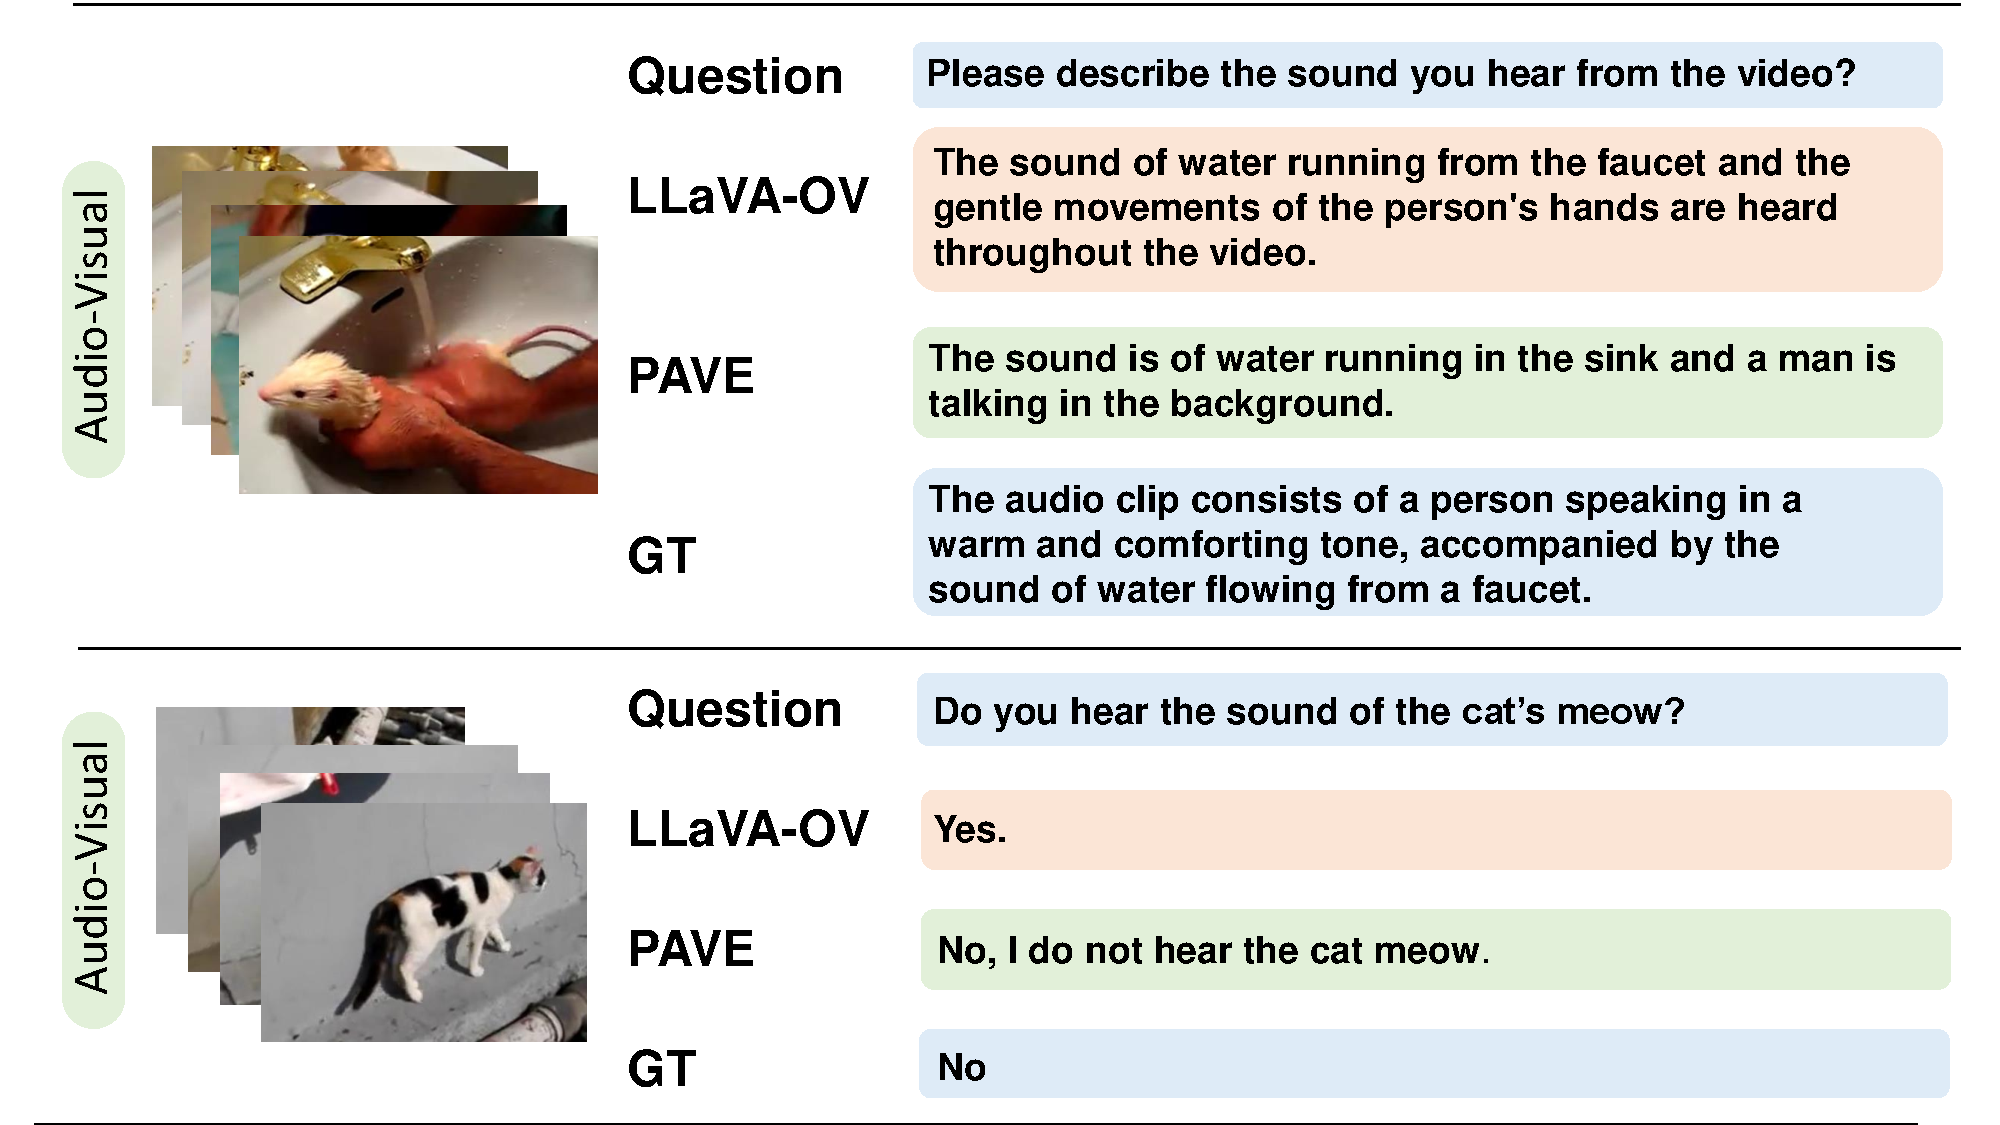
\includegraphics[width=0.8\linewidth]{figures/additional_qa_visualization.pdf}
%     % \vspace{-1em}
%     \caption{Additional visualization of audio-visual setting. We select online videos and ask question about the audio information. PAVE are able to understand the audio correctly instead of just inferring the sound from the visual information.}
%     \label{fig:additional_audio_visual}
%     % \vspace{-1em}
% \end{figure*}


\begin{figure*}[t!]
    \centering
    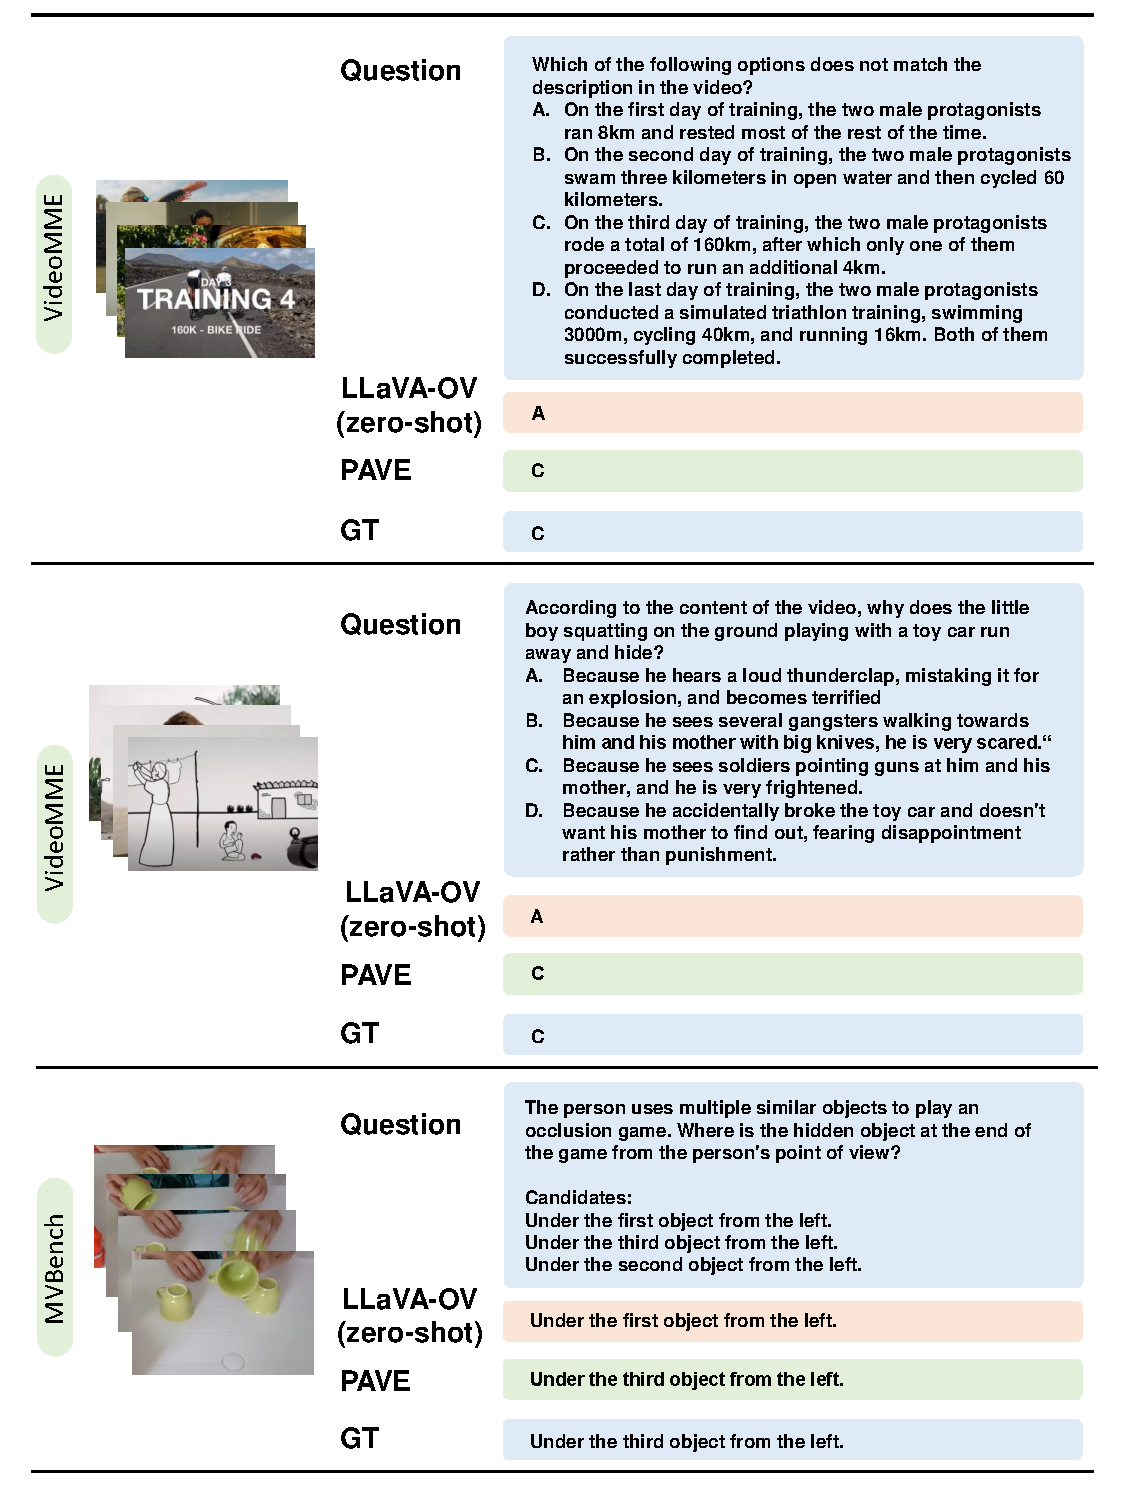
\includegraphics[width=0.75\linewidth]{figures/additional_general_qa_visualization.pdf}
    \vspace{-1em}
    \caption{Visualization of the QA results on enhanced video QA task. By making use of the video feature of the densely sampled video frames, PAVE captures more details in the video and thus improves the performance of video understanding.}
    \label{fig:enhanced_qa_visualization}
    \vspace{-1.5em}
\end{figure*}




% \section{Discussion and Future Works} \label{discussion}

% % \subsection{Discussion of training and using multiple patches}
% In the ablation study of the main paper, we investigate training multiple patches together. We provide additional experiment details and further discussion here.

% We use the enhanced video understanding patch (PAVE-7B model in Table~\ref{tab:general_video_understanding} of the main paper) in this experiment. Specifically, we employ the PAVE module from the enhanced video understanding setting and instantiate a new PAVE module with new LoRA weight for LLM to adapt the Video LLM to the setting where the audio and the densely sampled video frames serve as the side-channel information. 
% During training, we freeze the PAVE module from the enhanced video understanding setting so that the performance on the enhanced video understanding will not change while the new patch for audio-visual setting can benefit from the information in the densely sampled video frames.
% After training, we have two distinct patches: one for enhanced video understanding and another for audio-visual understanding. 
% During the inference in an audio-visual setting, we activate both patches (two PAVE modules) and the LoRA weight that was trained for the audio-visual setting. PAVE takes keyframes, high-framerate video, and audio as input.

% For the trained patches, while we can deploy them independently and regard each of them as a standalone model, we can also consider merging them into a single mixture-of-expert (MoE) model, with each task-specific patch as an expert, though this topic is already beyond the scope of this paper. This could be handled by modifying the LoRA and model wrapper to load multiple LoRA weights and PAVE modules at the same time. During inference, this MoE model routes an input to a task expert and activates its weights.
% A straightforward approach to implementing this routing mechanism is rule-based selection, where the patch is chosen based on the type of side-channel information available in a given sample. Future work could explore more advanced routing strategies that involve training the router to learn optimal patch selection.





